\section{Lower Bounds} \index{lower bound} \index{model of computation} \index{comparison model}

So far, we have been talking almost exclusively about how we can use different algorithms and data structures to solve certain problems as fast as possible. In this part, we will focus on proving certain problems cannot be solved as quickly as we might want. In other words, there is a limit to how good we can do. For example, in a comparison model, sorting can only be achieved at best in $\Omega(n \log n)$ time in the worst case.

\begin{definition}
    Let $P$ be a problem. The worst case complexity of problem $P$ is
    $$
    C(P) = \min \{ C_A \mid \text{$A$ is an algorithm that solves $P$} \}
    $$
    where $C_A:\; \N \to \N$ is the worst case complexity of algorithm $A$.
\end{definition}

We can prove the upper-bound of the complexity of a problem by giving a specific algorithm $A$ that solves $\Pi$, and faster algorithms give us smaller (tighter and better) upper bounds.

However, to prove that a problem has a certain lower bound, it is not enough to give an algorithm and say that we cannot do better. We have to show that every algorithm that solves $\Pi$ has a worst-case running time $\Omega(f(n))$, or equivalently, that there is no algorithm that solves $\Pi$ that runs in $o(f(n))$ time. To be more specific, we need to specify what kinds of algorithms we want to consider, which is formally known as model of computation. For example, the comparison model is one model that is used to solve sorting and searching problems.


Let $\mathcal{A}$ be a class of algorithms. The worst-case complexity of problem $P$ in class $\mathcal{A}$ is
$$
C(P) = \min \{ C_A \mid \text{$A \in \mathcal{A}$ is an algorithm that solves $P$} \}
$$
$\mathcal{A} \subseteq \mathcal{A}'$ implies that a lower bound on the worst-case complexity of $P$ in class $\mathcal{A}'$ is also a lower bound on the worst-case complexity of $P$ in class $\mathcal{A}$. In other words, lower bounds in more powerful models are better.

\section{Comparison Model}

In the comparison model, we consider all input items as black boxes, or more precisely, ADTs. The only operations allowed on the items are comparisons: $<, \leq, >, \geq, =$. Most searching and sorting algorithms we have been looking at so far use the comparison model: heap sort, merge sort, binary search and binary search tree, etc. In the comparison model, we count the number of comparisons and define it as the time cost of the algorithm.

\section{Comparison Tree}

\subsection{Intuition}

Any comparison algorithm can be viewed as a tree of all possible comparisons, the outcomes of the comparisons, and the resulting answer. This tree is called a decision tree. There is a different tree for each different input size.

For any particular $n$,
\begin{itemize}
    \item \textit{internal node} corresponds to a decision in the algorithm (in this case, comparisons)
    \item \textit{edge} corresponds to a possible outcome of the comparison denoted by the node
    \item \textit{leaf} corresponds to a possible answer (output) of the problem
    \item \textit{root-to-leaf path} corresponds to an execution of the algorithm
    \item \textit{length of the root-to-leaf path} corresponds to the time cost of the execution associated with that path
    \item \textit{height of the tree} (or depth of the deepest leaf) corresponds to the worst-case running time.
\end{itemize}


\subsection{Decision Tree for Searching}

Consider a comparison tree for the binary search algorithm. An example is shown below for binary search for $x$ in $A[1\ldots 3]$ using only $\leq$ comparisons and outputs $i$ such that $x=A[i]$ or 0 if no such element exists.

The average case complexity the algorithm is the expected path length, that is the weighted average depths of the leaves.
$$
\sum_{\ell} (\attrib{\ell}{depth}) \cdot \Prob [\text{input leads to $\ell$}]
$$

Another example is for searching in $[2,3,5,7,11,13,17,19]$ using $<$ and $=$ comparisons. 

\hfill

\begin{figure}[htbp]
    \centering
    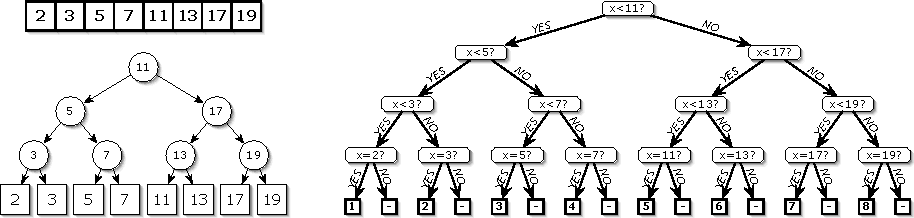
\includegraphics[width=\linewidth]{figures/binary_search_decision_tree.pdf}
    \caption{Decision tree for searching the array containing $[2,3,5,7,9,11,13,17,19]$.}
    \label{fig:sorting-tree-2}
\end{figure}

\subsection{Decision Tree for Sorting}